\documentclass{beamer}
\usepackage[utf8]{inputenc}
\usepackage{musicography}
\usepackage{graphicx}



%% doc deets
\title{The Order of Mathematistry}
\subtitle{Queering metascience with mathematics}
\titlegraphic{
%\vspace{-5cm}
\begin{tikzpicture}[scale=0.8]


% images
\usepackage[export]{adjustbox}
\usepackage{caption}

% nodes
\node [ style = hassenode] (f) {};
\node[style = hassenode] (g) at (-1, -1) {};
\node [style = hassenode] (h) at (1, -1) {};
\node [style = hassenode, gray] (i) at (0, -2) {};

%  edges
\draw [dotted] (f) to (g);
\draw (g)  to (i);
\draw [dotted] (i) to (h);
\draw (h) to (f);
%\vspace{5cm}
\end{tikzpicture}
}
\author{Charles T. Gray^{\musEighth}\\ Hannah Fraser, Hien Nguyen, \\Elise Gould, and Danielle Navarro}
\institute{\musEighth\ Reproducibility team, The repliCATS Project \\Interdisciplinary Metaresearch Group, University of Melbourne}

\date{February 2020}


% general packages
\usepackage{amssymb, amsthm, amsmath}

% biblio
\usepackage[url=false]{biblatex}
\addbibresource{references.bib}
%\renewcommand*{\bibfont}{\scriptsize}
\renewcommand*{\bibfont}{\tiny}

% itemised list
\usepackage{enumitem}

% tikz
\usepackage{tikz}
\usetikzlibrary[shapes,arrows]
\tikzset{hassenode/.style={circle,draw}}

% code macros
\newcommand{\code}[1]{\texttt{#1}}
\newcommand{\package}[1]{\texttt{#1::}}

% fix hyphenation issues
\usepackage[british]{babel} % hopefully this fixes some of the hyphenation issues
\hyphenation{re-pro-du-ci-bility}
\hyphenation{pre-reg-istration}


% beamer specs
\beamertemplatenavigationsymbolsempty
\setbeamertemplate{footline}[frame number]

\usefonttheme{serif}
\setbeamercolor*{structure}{fg= darkgray} 

%\setbeamercolor*{palette tertiary}{fg=black,bg=black!10} 
%\setbeamercolor*{palette quaternary}{fg=black,bg=black!10} 

%\setbeamercolor*{lower separation line head}{bg=orange} 
\AtBeginSection[]{\frame{\frametitle{Outline}%
\tableofcontents[currentsection,hideothersubsections]}}%

\usebackgroundtemplate{
\includegraphics[width=\paperwidth,height=\paperheight]{parchment.jpg}}

% theorem environment
\usepackage{thmtools}

\declaretheoremstyle{qthmstyle}
\declaretheorem[style=qthmstyle,name=Proposition]{proposition}
\declaretheorem[style=qthmstyle,name=Definition]{defn}
%\declaretheorem[style=qthmstyle,name=Lemma]{lemma}
%\declaretheorem[style=qthmstyle,name=Corollary]{corollary}




%%
\begin{document}



% title frame
\begin{frame}
\maketitle
\end{frame}

\section{A value judgement is, after all, an order}


\begin{frame}{Queering literature}

\begin{centering}
\begin{columns}

\begin{column}{0.5\textwidth}


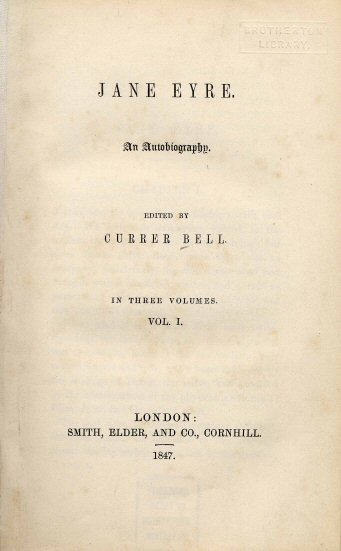
\includegraphics[scale=1.2]{Jane_Eyre_title_page.jpg}
\medskip

\small{
\emph{Jane Eyre}, 1847

\medskip

Charlotte Bront\"e~\cite{bronte2000jane}
}

\end{column}

\begin{column}{0.5\textwidth}



\includegraphics[scale=0.55]{JeanRhys_WideSargassoSea.jpg}
\medskip

\small{
\emph{Wide Sargasso Sea}, 1966

\medskip

Jean Rhys~\cite{rhys1992wide}
}


\end{column}

\end{columns}

\begin{flushright}
\tiny{Image sources: Wikipedia.}
\end{flushright}


% \begin{flushright}
% 
\includegraphics[scale=0.6]{JeanRhys_WideSargassoSea.jpg}

% \tiny{Image source: Wikipedia}
% \end{flushright}

% \emph{Wide Sargasso Sea}, Jean Rhys, 1966

% \bigskip
\end{centering}

\end{frame}

\begin{frame}{Queering metascience}

    \begin{quote}
        So let’s build an open and reproducible science as a queer reimagining of science and not a small perturbation of the world that is. Such a system will never be perfect. 
    \end{quote}

\begin{flushright}
-- Dan Simpson~\cite{simpson_what_2019}    
\end{flushright}
    
\end{frame}

\begin{frame}{Preregistration is redundant, at best}

The Centre for Open Science defines preregistration as `specifying' the research plan in advance~\cite{centre_for_open_science_preregistration_2020}.

\bigskip

2019: Preregistration is Hard, and Worthwhile, Nosek \emph{et al.}~\cite{nosek_preregistration_2019}

\bigskip

2019: Is Preregistration Worthwhile? Szollosi \emph{et al.}~\cite{szollosi_preregistration_2019}

\bigskip

\begin{quote}
The diagonisticity of statistical tests depend entirely on how well statistical models map onto underlying theories, and so improving statistical techniques does little improve theories \underline{when the mapping is weak}~\cite{szollosi_preregistration_2019}.
\end{quote}

    
\end{frame}

\begin{frame}{Mathematistry}
Navarro, a mathematical scientist specialising in psychology, redefines Box's term \textbf{mathematistry}~\cite{box_science_1976} to 

\bigskip

\begin{quote}
`describe using formal tools to define a statistical problem that differs from the
scientific one, solving the redefined problem, and declaring the scientific concern addressed'~\cite{navarro_between_2018}.    
\end{quote}

\bigskip

We will think of \textbf{mathematistry} as the measure of strength of mapping to describe \underline{when the mapping is weak}~\cite{szollosi_preregistration_2019}.


\end{frame}

%%% Order
\begin{frame}{A value judgement is, after all, an order}
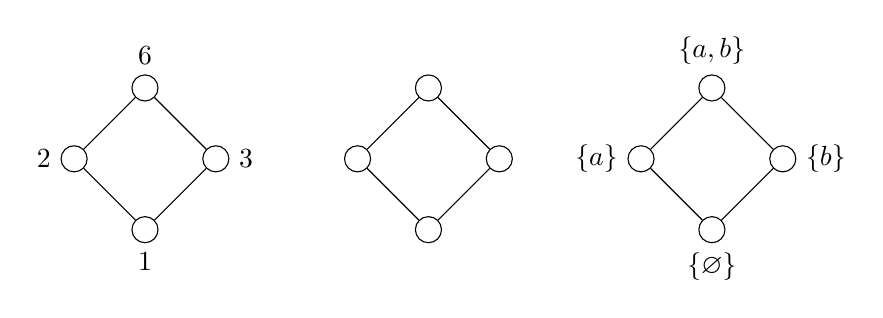
\begin{tikzpicture}[scale = 0.9]

\begin{scope}[xshift=0cm]

  % nodes

  \node [ style = hassenode, label=above:6] (f) {};
  \node[style = hassenode, label=left:2] (g) at (-1, -1) {};
  \node [style = hassenode, label=right:3] (h) at (1, -1) {};
  \node [style = hassenode, label=below:1] (i) at (0, -2) {};

  %  edges
  \draw [] (f) to (g);
  \draw (g)  to (i);
  \draw [] (i) to (h);
  \draw (h) to (f);

  \end{scope}

\begin{scope}[xshift=4cm]

% nodes
\node [ style = hassenode] (f) {};
\node[style = hassenode] (g) at (-1, -1) {};
\node [style = hassenode] (h) at (1, -1) {};
\node [style = hassenode] (i) at (0, -2) {};

%  edges
\draw [] (f) to (g);
\draw (g)  to (i);
\draw [] (i) to (h);
\draw (h) to (f);

\end{scope}

\begin{scope}[xshift=8cm]

% nodes

  \node [ style = hassenode, label=above:{\(\{a,b\}\)}] (f) {};
  \node[style = hassenode, label=left:{\(\{a\}\)}] (g) at (-1, -1) {};
  \node [style = hassenode, label=right:{\(\{b\}\)}] (h) at (1, -1) {};
  \node [style = hassenode, label=below:{\(\{\varnothing\}\)}] (i) at (0, -2) {};

%  edges
\draw [] (f) to (g);
\draw (g)  to (i);
\draw [] (i) to (h);
\draw (h) to (f);

\end{scope}

\end{tikzpicture}
\end{frame}



%%%  Heuristics

\section{Heuristics of mathematistry}


\begin{frame}{Heuristics of mathematistry}
\begin{center}
\begin{tikzpicture}[scale = 0.9]
\begin{scope}

%  nodes
\node [style = hassenode] (a) at (0,0) {};
\node [style = hassenode] (b) at (0,-2) {};

% edges
\draw (a) to (b);
\end{scope}

%\end{tikzpicture}

%\begin{tikzpicture}

\begin{scope}[xshift=4cm]

% nodes
\node [style = hassenode, gray] (c) at (0,0) {};
\node [style = hassenode] (d) at (0,-1) {};
\node [style = hassenode, gray] (e) at (0, -2) {};

% edges
\draw [dotted] (c) to (d);
\draw [dotted] (d) to (e);
\end{scope}

\begin{scope}[xshift=8cm]

% nodes
\node [ style = hassenode] (f) {};
\node[style = hassenode] (g) at (-1, -1) {};
\node [style = hassenode] (h) at (1, -1) {};
\node [style = hassenode, gray] (i) at (0, -2) {};

%  edges
\draw [dotted] (f) to (g);
\draw (g)  to (i);
\draw [dotted] (i) to (h);
\draw (h) to (f);

\end{scope}

\end{tikzpicture}
\end{center}


% \end{frame}

%\begin{frame}


%\onslide<2> {

\small{
$$
h: C \times M \to \begin{cases}
                \{0, 1\} & \text{if heuristic categorises as effective or not;}\\
                [0, 1] & \text{if heuristic measures efficacy on a spectrum;}\\
                H & \text{if heuristic categorises efficacy otherwise},
            \end{cases}
$$
}
%}

\end{frame}


\begin{frame}{Heuristics of mathematistry}

Let $C$ denote the set of all possible \textbf{scientific claims} for which we might provide evidence of, with a scientific method or procedure.

\bigskip

Let $M$ denote the set of all possible \textbf{scientific methods} that can be used to provide evidence of scientific claims.

\bigskip 

The product $C \times M$ denotes the collection of possible \textbf{pairings of claim and methodology}. 

\end{frame}

\begin{frame}{Heuristic of mathematistry}

\begin{definition} A \textbf{heuristic $h$ of mathematistry} measures the efficacy of a pairing $(c,m)$ of scientific claim $c \in C$, and method  $m \in M$ of providing evidence of that claim, measuring how effective method $m$ is at scientifically informing claim $c$.

\vspace{1cm}

We denote $\mathbb H$ to be the set of all possible heuristics of mathematistry. For a heuristic $h$ in $\mathbb H$, we define the value $h(c,m)$ as the \textbf{measure of mathematistry} of pairing $(c,m)$ under heuristic $h$.
\end{definition}

\end{frame}

\begin{frame}{A value judgement on \emph{good enough}~\cite{wilson_good_2017} science}

\begin{center}
\begin{tikzpicture}[scale = 0.7]
\begin{scope}

%  nodes
\node [style = hassenode, label=above right:{$\top$}] (a) at (0,0) {};
\node [style = hassenode, label=below right:{$\bot$}] (b) at (0,-2) {};

% edges
\draw (a) to (b);
\end{scope}

%\end{tikzpicture}

%\begin{tikzpicture}

\begin{scope}[xshift=4cm]

% nodes
\node [style = hassenode, gray, label=above right:{\textcolor{gray}{$\top$}}] (c) at (0,0) {};
\node [style = hassenode] (d) at (0,-1) {};
\node [style = hassenode, gray,label=below right:{\textcolor{gray}{$\bot$}}] (e) at (0, -2) {};

% edges
\draw [dotted] (c) to (d);
\draw [dotted] (d) to (e);
\end{scope}

\begin{scope}[xshift=8cm]

% nodes
\node [ style = hassenode, label=above right:{$\top$}] (f) {};
\node[style = hassenode] (g) at (-1, -1) {};
\node [style = hassenode] (h) at (1, -1) {};
\node [style = hassenode, gray, label=below right:{\textcolor{gray}{$\bot$}}] (i) at (0, -2) {};

%  edges
\draw [dotted] (f) to (g);
\draw (g)  to (i);
\draw [dotted] (i) to (h);
\draw (h) to (f);

\end{scope}

\end{tikzpicture}
\end{center}    

\bigskip

For a heuristic $h$ to be a member of $\mathbb H$, there must exist a scientific method $m$, and two distinct scientific claims we might reasonably pair $m$ with, $c_1$ and $c_2$, such that
$$
h(c_1,m) <  h(c_2,m)
$$
or, conversely, there must exist distinct methods, $m_1$ and $m_2$, such that, for a claim $c$, we have
$$
h(c, m_1) < h(c, m_2).
$$



\end{frame}



%%% Order operation

\begin{frame}{A relational operator of mathematistry}

\begin{definition}\label{def:om}
Let $(c_1, m_1) \to_h (c_2, m_2)$ if and only if $h(c_1, m_1) \leqslant h(c_2, m_2)$ under heuristic $h$ of mathematistry.
\end{definition}


    
\end{frame}


\section{The order of mathematistry}

%%% Order definition

\begin{frame}{Order}

To be considered an order, $\to_h$ must satisfy three properties~\cite{davey_introduction_2002-1}.

\vspace{1.5cm}

\begin{defn}\label{def:order}
A binary relation $\leqslant$ on set $P$ is an \textbf{order} if, for all $x, y, z \in P$, we have
\begin{enumerate}[label=(\roman*)]
    \item $x \leqslant x$,
    \item $x \leqslant y$ and $y \leqslant x$ implies $x = y$,
    \item $x \leqslant y$ and $y \leqslant z$ imply $x \leqslant z$.
\end{enumerate}

\end{defn}

\end{frame}


%%% Order definition

\begin{frame}{Order}

\begin{description}%[label=(\roman*)]
    \item[(i) reflexivity] $x \leqslant x$,
    \item[(ii) antisymmetry] $x \leqslant y$ and $y \leqslant x$ implies $x = y$,
    \item[(iii) transitivity] $x \leqslant y$ and $y \leqslant z$ imply $x \leqslant z$.
\end{description}

\vspace{1.5cm}

When a binary relation satisfies (i) reflexivity and (iii) transitivity, but not (ii) antisymmetry, we say it is a \textbf{quasi-order}.


 \end{frame}

\begin{frame}{A quasi-order of mathematistry}
 
 \begin{definition}
 When a binary relation satisfies (i) reflexivity and (iii) transitivity, but not (ii) antisymmetry, we say it is a \textbf{quasi-order}.
 \end{definition}
 
\vspace{1cm}
 
 Let $\mathcal X \subseteq C \times M$ denote the subset $\mathcal X$ of reasonable pairings $C \times M$ of claims and methods.
 
 \bigskip

    \begin{lemma}\label{lem:quasi}
The relation $\to_h$ is a quasi-order on $\mathcal X$.
\end{lemma}




\end{frame}

%%%% Order of Mathematistry
\begin{frame}{The Order of Mathematistry}
    
\end{frame}

%%% biblio

\section*{References}

\begin{frame}[allowframebreaks]{References}
\printbibliography
\end{frame}

\end{document}
